\documentclass[a4paper]{jpconf}
\usepackage{graphicx}
\usepackage{iopams}
\usepackage{hyperref}
\begin{document}
\title{Federating Distributed Storage For Clouds In ATLAS}

\author{Berghaus~F, Casteels~K, Driemel~C, Ebert~M, Galindo~F, Leavett-Brown~C, Paterson~M, Seuster~R, Sobie~R, Tafirout~R, Taylor~R~P}

\address{Frank~Berghaus, G07810, CERN, CH-1211 Geneva 23,  Switzerland}

\ead{frank.berghaus@cern.ch}

\begin{abstract}
Input data for applications that run in cloud computing centres can be stored at distant repositories, often with multiple copies of the popular data stored at many sites. Locating and retrieving the remote data can be challenging, and we believe that federating the storage can address this problem. A federation would locate the closest copy of the data on the basis of GeoIP information. Currently we are using the dynamic data federation DynaFed~\cite{dynafed} software solution developed by CERN IT. DynaFed supports several industry standards for connection protocols like Amazon's S3, Microsofts Azure, as well as WebDAV and HTTP. Protocol dependent authentication is hidden from the user by using their X509 certificate. We have setup an instance of DynaFed and integrated it into the ATLAS Data Distribution Management system. We report on the challenges faced during the installation and integration. We have tested ATLAS analysis jobs submitted by the PanDA production system and we report on our first experiences with its operation.
\end{abstract}

\section{Introduction}
Our goal is run data-intensive applications on globally distributed opportunistic resources that have no local grid storage. The ATLAS experiment leverages a globally distributed system of infrastructure as a service clouds, such as Amazon's Web Services, or the Compute Canada, and CERN OpenStack. These resources are integrated into the ATLAS distributed computing system using two cloud scheduler~\cite{cloud-scheduler} instances: one at the University of Victoria and one at CERN. These IaaS resources are used opportunistically, and do not support any local grid infrastructure.

The workflows executed by high energy physics experiments often demand large volumes of input data or produce a significant volume of output data. We aim to use a data federation, such as DynaFed, to redirect the applications running on opportunistic resources to the optimal storage endpoint to retrieve input or deposit output data.

\section{Conceptual Design}
The ATLAS experiment leverages the resources of the Worldwide LHC Computing Grid, WLCG~\cite{wlcg}. The computer centres that are part of the WLCG and support that ATLAS experiment each host some of the experiment data and simulated events. They provide a global storage infrastructure. While the central ATLAS computing infrastructure uses purpose specific protocols to access the content of these grid storage elements, they may be accessed using standard protocols such as WebDAV, HTTP, and NFS. Figure~\ref{fig:conceptual-design} shows how DynaFed could appear to present the entire ATLAS data catalog by unifying the namespaces of attached storage elements.

\begin{figure}
  \centering
  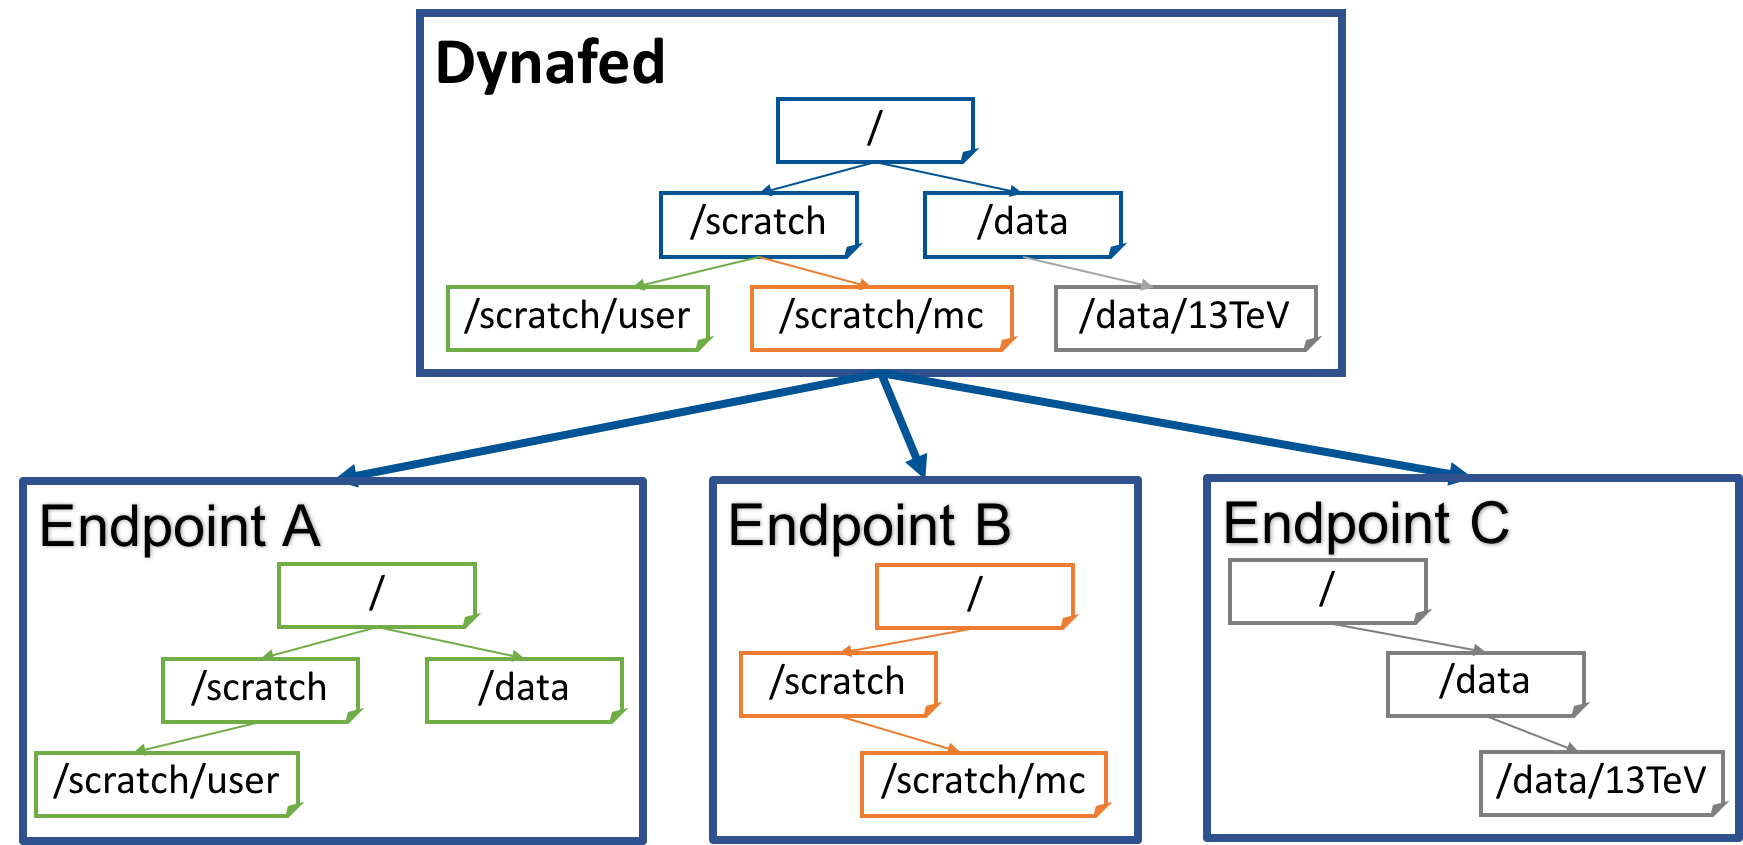
\includegraphics[width=\textwidth]{conceptual-design.png}
  \caption{The dynamic federation is cpnnected to multiple endpoints. Each endpoint may be a file system or an object store accessible using the a protocol which allows redirection. The dynamic federation appears to provide a namespace that is a union of all the namespaces of the endpoints. That namespace is presented as a familiar directory structure on the same protocols as exposed by the endpoints.}
  \label{fig:conceptual-design}
\end{figure}

Cloud storage systems are object stores that expose a well defined interface over HTTP and WebDAV. DynaFed also allows the inclusion of these cloud storage into the a grid system. DynaFed implements authentication through public key infrastructure with grid extensions~\cite{voms} and translates this authentication to authorize access to the cloud storage systems which each have their own authentication and authorization paradigms. Thus a grid user or application authenticates to DynaFed using grid credentials and is forwarded to a pre-signed URL that permits, for a limited time, access to the cloud storage system.

\section{Data Access}
The DynaFed instance regularly polls all connected endpoints to determine if they are reachable. Should an endpoint become unresponsive no requests will be forwarded to it until it responds again. This dynamically adjusts for storage endpoint failures and should increase the stability of the storage system as a whole.

\begin{figure}
  \centering
  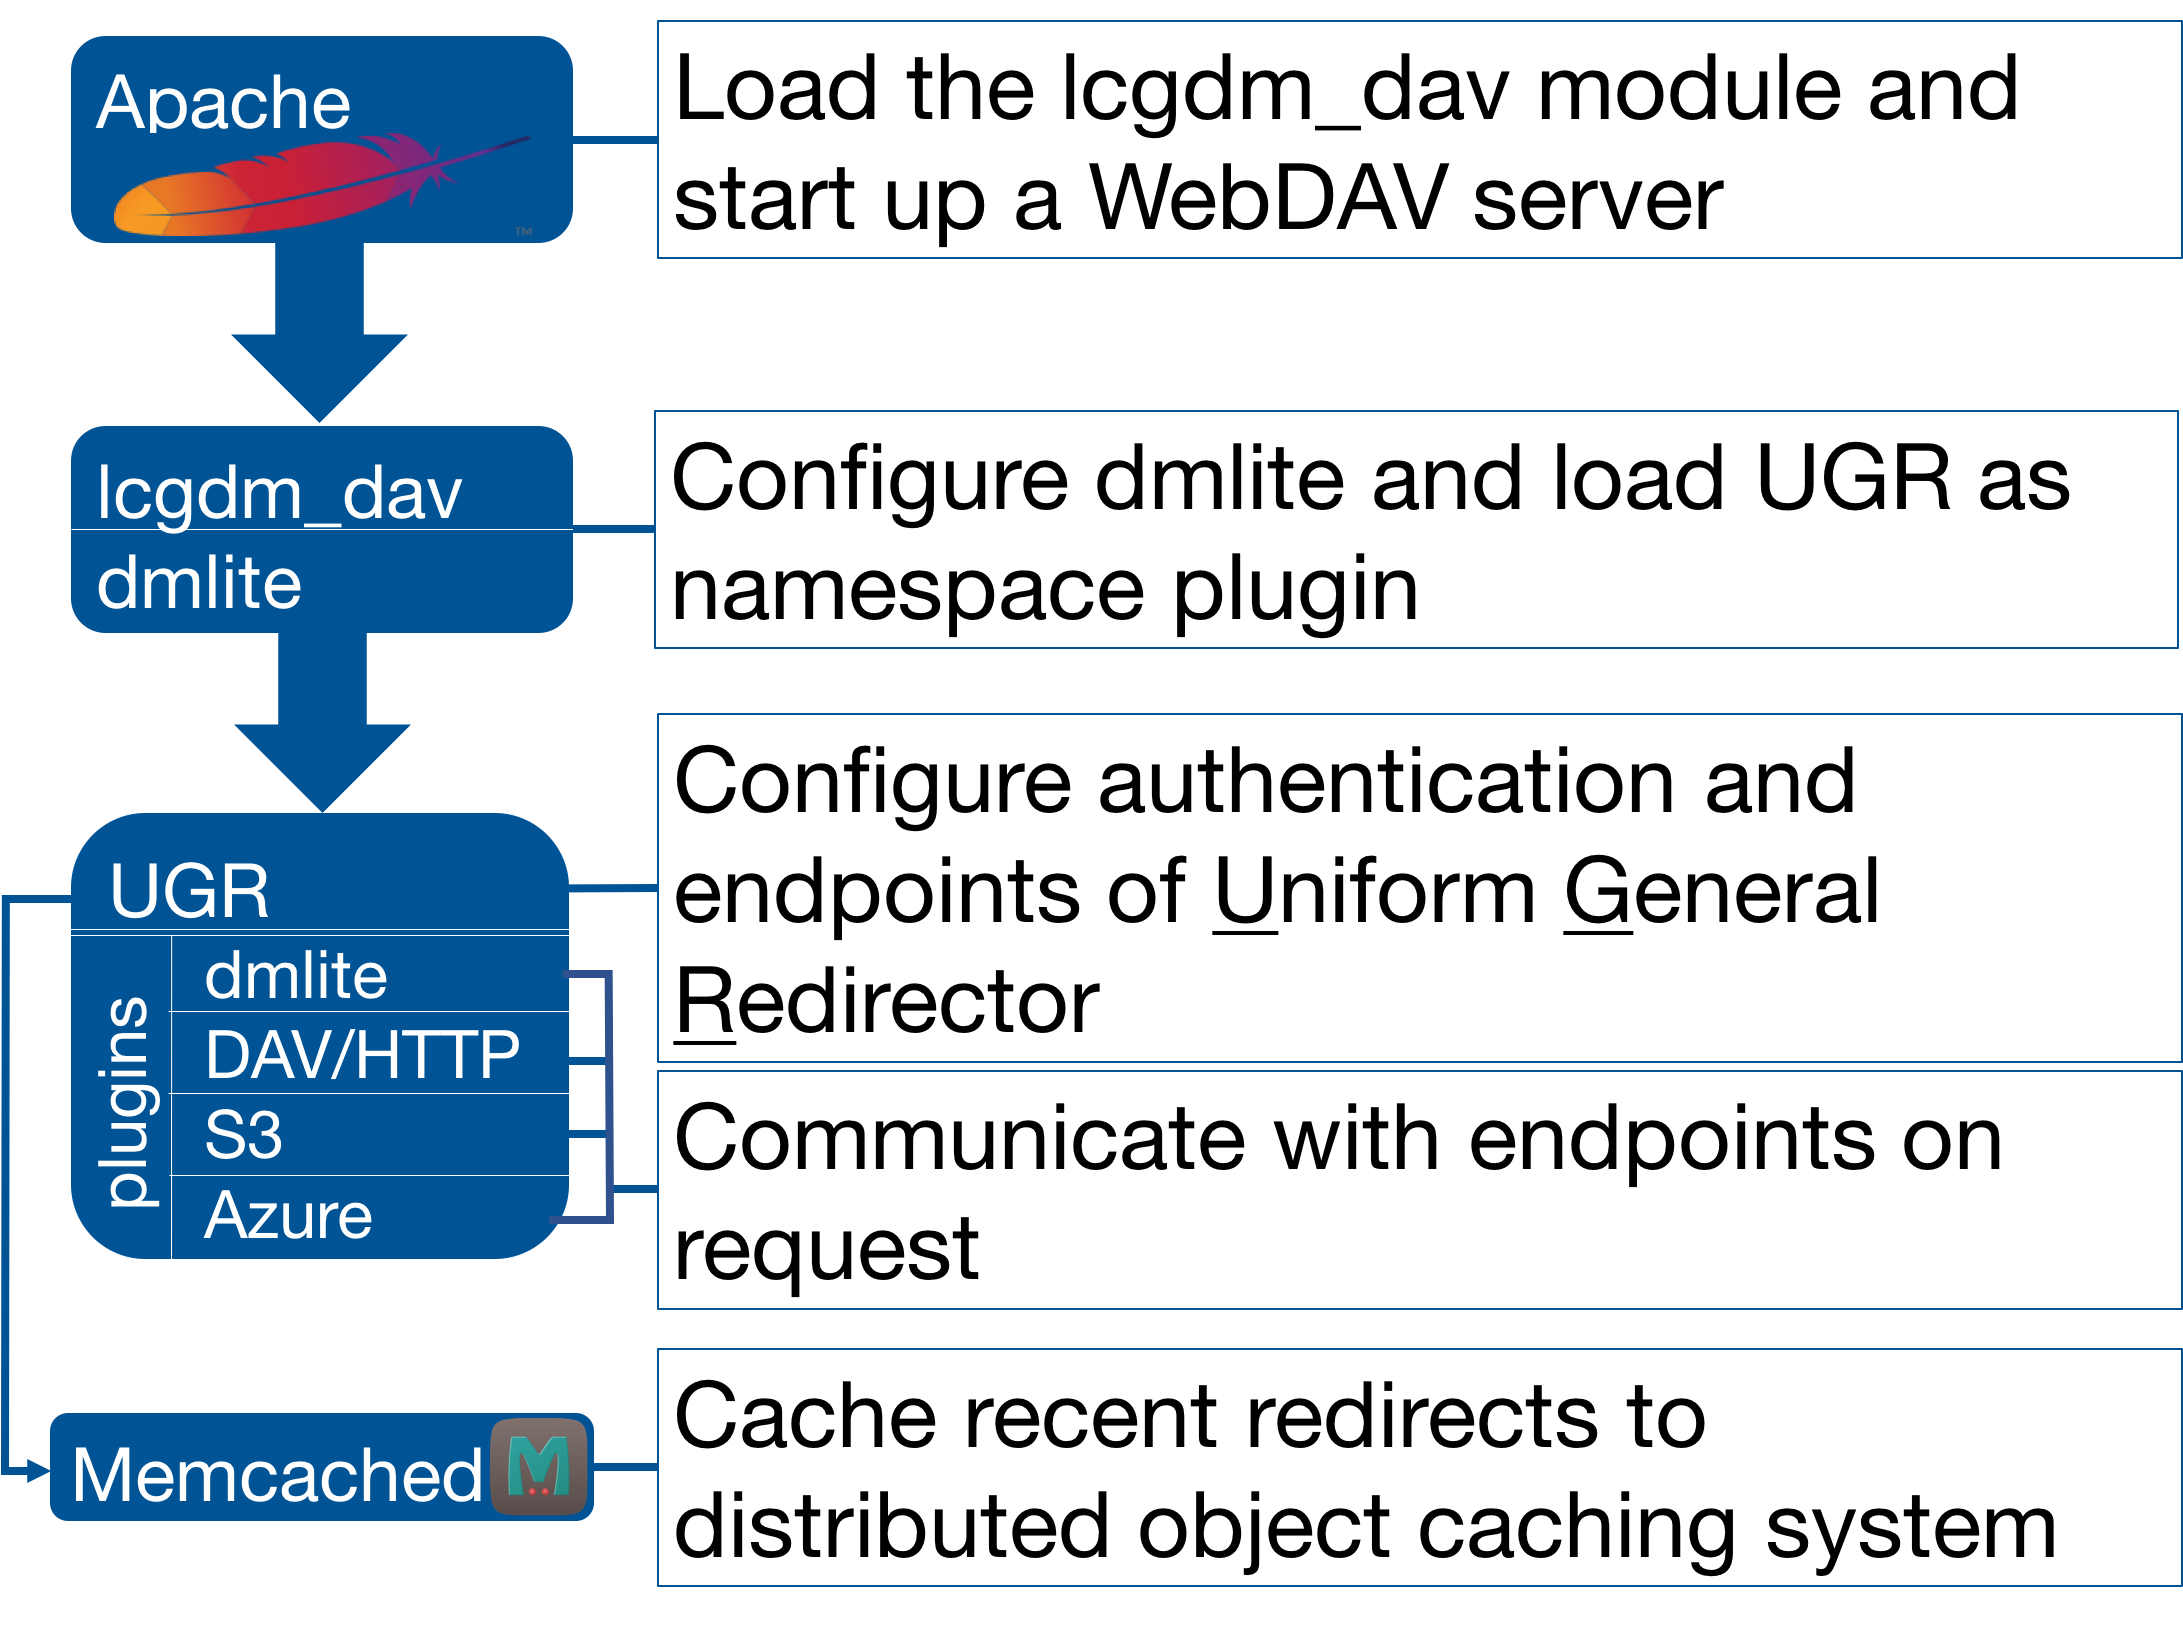
\includegraphics[width=\textwidth]{dynafed-arch.png}
  \caption{The dynamic web federation is an apache we server running the LCGDM implementation of WebDAV. The namespace generally managed by LCGDM has been replaced by the uniform general redirector which translates the requests to the web file system to the connected endpoints. The endpoint module handle the communicate with the connected endpoints. All requests are cached in memory on the server as well as in a second level cache which may be shared across multiple load-balanced servers.}
  \label{fig:dynafed-arch}
\end{figure}

Figure~\ref{fig:dynafed-arch} illustrated the task division in the dynamic federation handle client requests. When the dynamic federation receives a requests for a while in it's namespace the client is authenticated. Once the request has been authenticated the name is looked up in the cached. If a cached entry exists that entry is returned. If the cache does not contain an entry for the queried file the name of the file is translated to each of the endpoints and the endpoints are queried. The federation waits for a response from all endpoints up to some timeout. The response is cached and the client is redirected to the geographically closest copy of the data. It is also possible to query a metalink which returns a XML list of all copies of the queried file. In the future we wish to implement chunked downloads from multiple locations using this metalink and the area2c copy tool. Should the client make a request to write dynafed redirects the client to the geographically closest writeable storage element.


\section{Application Workflow}
The goal of this project is to integrate the dynamic federation into the ATLAS and Belle-II distributed computing and data management systems. Here we will focus on the ATLAS system since the integration into PanDA~\cite{panda} and Rucio is more mature.

Currently ATLAS distributed computing takes advantage of volunteer resources~\cite{boinc} and opportunistic cloud resources. The cloud resources are used as the testbed for this work, but the results will be useful for both and hopefully more. Cloud resources are included into ATLAS distributed computing using the cloud scheduler technology as illustrated in figure~\ref{fig:atlas-cloud}. A cloud scheduler system executes ATLAS workloads on globally distributed cloud resources. The virtual machine instances that execute the ATLAS workload are configured to connect to DynaFed for input and output data.

Storage backends from the University of Victoria and TRIUMF in Canada as well as the University of Edinburough and CERN in Europe are connected to the dynamic federation. Input data was copied to the federation using the file transfer service~\cite{fts3} at CERN. The data sets were manually registered with Rucio. With the input datasets registered we executed functional tests on virtual machine workers that ran on the CERN OpenStack cloud, retrieved their input from a CephS3 interface at CERN through the dynamic federation, and uploaded their logs and results to the same storage upon completion.

\begin{figure}
  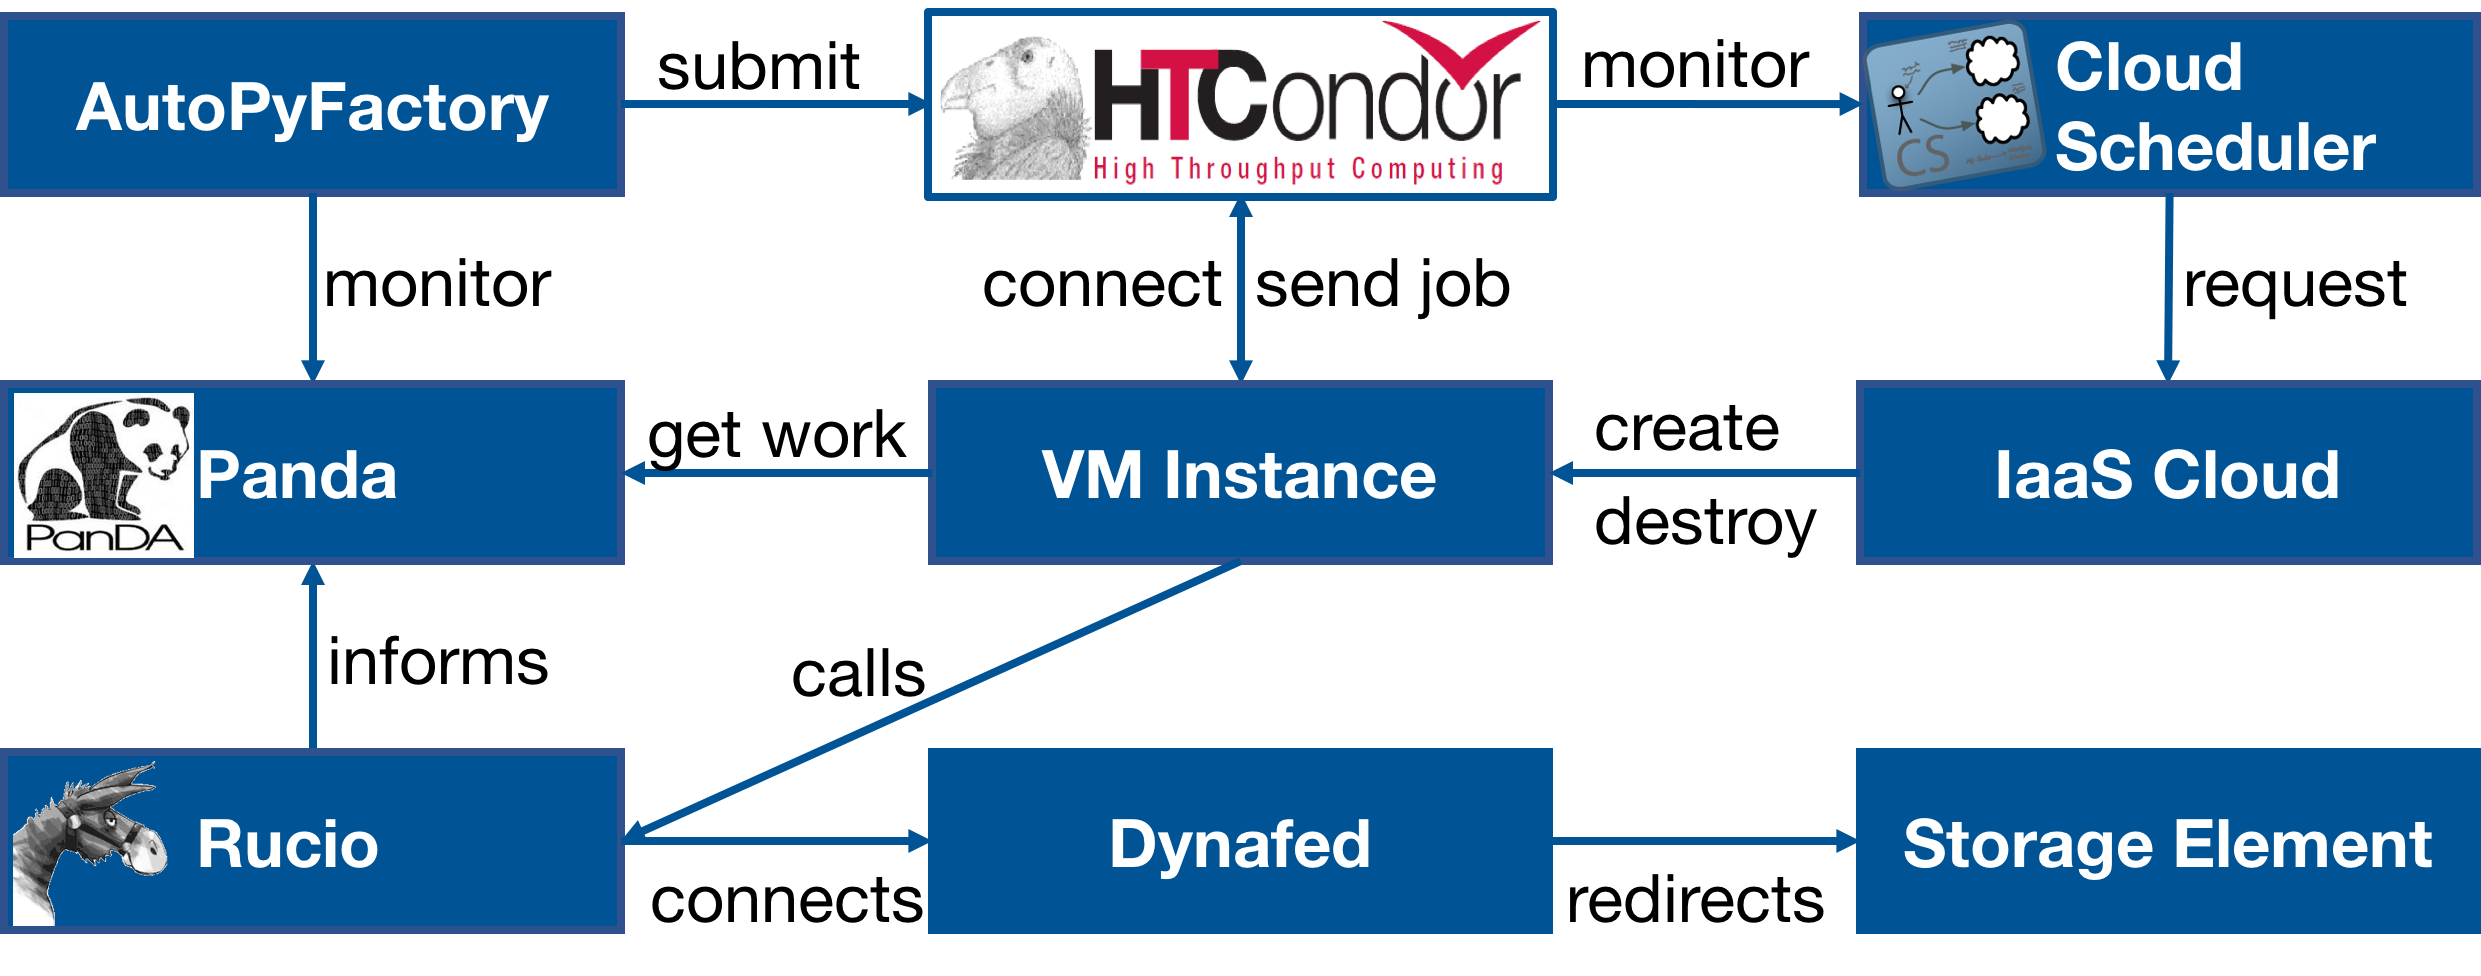
\includegraphics[width=\textwidth]{atlas-cloud-system.png}
  \caption{A client (AutoPyFactory or Harvester) submit pilot wrapper scripts to an HTCondor queue. The queue is monitored by a cloud scheduler. The cloud scheduler makes requests to connected cloud interfaces in response to load on the queue. The cloud infrastructures create virtual machine instances and provide user-data to cloud-init running in the virtual machines for configuration. The VM instances are configured to connect to the condor and start consuming jobs from the queue. The pilot wrapper scripts run on the virtual machines and download the pilot which drains tasks from a PanDA queue. The pilot uses Rucio to download input data and upload results. Rucio is configured to contact the dynamic federation via WebDAV. The federation forwards Rucio to the closest available storage.}
  \label{fig:atlas-cloud}
\end{figure}

For full integration of cloud storage into the ATLAS distributed data management some additional development is necessary: bulk transfers negotiated between storage endpoints using the HTTP and WebDAV protocols must be fully supported and the data management system must be able to parse the checksums of files on cloud storage.

 % The ATLAS experiment uses the adler32 algorithm~\cite{adler32} because it is fast and can perform a checksum of a file copied over multiple streams, while being reliable to ensure the integrity of the ATLAS data catalogue. Cloud storage have chosen to use the well proven MD5 checksum algorithm~\cite{md5}. To fully integrate cloud storage solution in the operating ATLAS distributed data management system we will integrate add the MD5 checksum for files on cloud storage systems. The protocol by which grid and cloud storage notify the client of the file checksum is different also: cloud storage includes the MD5 digest as the value of the ETag in the return header of get and put requests. Grid storage responds with the checksum digest to a header containing the name of the checksum algorithm in the 'Request-Digest' field.


\section{Summary}
It was shown that ATLAS functional tests can retrieve and deposit their data on a cloud storage accessed over the WebDAV protocol using a dynamic federation. The functional tests ran on virtual machine instances in a cloud infrastructure and could be scheduled anywhere in the distributed cloud system currently running as part of the ATLAS production system. Further development is necessary to execute production jobs against the dynamic federation and for the usage with the Belle-II experiment and thereby the DIRAC workload management system.


%\section*{Acknowledgments}
\ack
This work was made possible because of the gracious help of many people: the CERN storage team, specifically Fabrizio Furano for their help with the dynamic federation and Dan van~der~Ster with the Ceph S3 cluster, the ATLAS DDM team, especially Mario Lassnig and Cedric Serfon for integrating the dynamic federation with Rucio, and Alessandro di~Girolamo and Ivan Glushkov for their help with the integration into ATLAS distributed computing.

This work was made possible by funding from the (funding agency?).


\section*{References}
\begin{thebibliography}{9}
\bibitem{dynafed}
  Furano~F {\it et al}
  2017
  Dynafed
  \url{http://cern.ch/lcgdm/dynafed-dynamic-federation-project}
\bibitem{cloud-scheduler}
  Gable~I {\it et al}
  2017
  Cloud Scheduler
  \url{http://cloudscheduler.org}
\bibitem{wlcg}
  Bird~I
  2011
  %``Computing for the Large Hadron Collider''
  {\it Ann.\ Rev.\ Nucl.\ Part.\ Sci.\ } {\bf 61} 99
  %doi:10.1146/annurev-nucl-102010-130059
\bibitem{voms}
  Foster~I, Kesselman~C and Tuecke~S
  2001
  ``The Anatomy of the Grid: Enabling Scalable Virtual Organizations''
  {\it International Journal of Supercomputer Applications}
  %\url{http://www.globus.org/alliance/publications/papers/anatomy.pdf}
\bibitem{panda}
  T.Maeno {\it et al}
  2017
  PanDA
  \url{http://www.pandawms.org}
\bibitem{boinc}
  Cameron D and Wu W
  2017
  LHC@home
  \url{http://lhcathome.web.cern.ch}
\bibitem{fts3}
  CERN IT-ST
  2017
  FTS3
  \url{http://fts3-service.web.cern.ch/}
\bibitem{adler32}
  Deutsch P and Gailly J-L
  1996
  ``ZLIB Compressed Data Format Specification Version 3.3''
  IETF RFC 1950
\bibitem{md5}
  Rivest R
  1992
  ``The MD5 Message-Digest Algorithm''
  IETF RFC 1321


\end{thebibliography}

\end{document}
